

% -------------------------------------------------------------------
% abnTeX2: Modelo de Trabalho Academico (tese de doutorado, 
% dissertacao de  mestrado e trabalhos monograficos em geral)
% em conformidade com  ABNT NBR 14724:2011:
% -------------------------------------------------------------------
%obs. os novos arquivos a serem criados e adicionados
%devem ter a codificação UTF-8.
% --------------------------------------

% configurações do documento com padrões
% ABNT, (usando o template ABNTex2).
%\include{configuracoesDoDocumento}

\documentclass[
	% -- opções da classe memoir --
	12pt,				% tamanho da fonte
	openright,			% capítulos começam em pág ímpar (insere página vazia caso preciso)
    %	twoside,			% para impressão em verso e anverso. Oposto a oneside
	oneside,
	a4paper,			% tamanho do papel. 
	% -- opções da classe abntex2 --
	%chapter=TITLE,		% títulos de capítulos convertidos em letras maiúsculas
	%section=TITLE,		% títulos de seções convertidos em letras maiúsculas
	%subsection=TITLE,	% títulos de subseções convertidos em letras maiúsculas
	%subsubsection=TITLE,% títulos de subsubseções convertidos em letras maiúsculas
	% -- opções do pacote babel --
	english,			% idioma adicional para hifenização
	french,				% idioma adicional para hifenização
	spanish,			% idioma adicional para hifenização
	brazil				% o último idioma é o principal do documento
	]{abntex2}

% ---
% Pacotes básicos 
% ---
\usepackage{lmodern}			% Usa a fonte Latin Modern			
\usepackage[T1]{fontenc}		% Selecao de codigos de fonte.
\usepackage[utf8]{inputenc}		% Codificacao do documento (conversão automática dos acentos)
\usepackage{lastpage}			% Usado pela Ficha catalográfica
\usepackage{indentfirst}		% Indenta o primeiro parágrafo de cada seção.
\usepackage{color}				% Controle das cores
\usepackage{graphicx}			% Inclusão de gráficos
\usepackage{microtype} 			% para melhorias de justificação

% ---
		
% ---
% Pacotes adicionais, usados apenas no âmbito do Modelo Canônico do abnteX2
% ---
%\usepackage{lipsum}				% para geração de dummy text
% ---

% ---
% Pacotes de citações
% ---
\usepackage[brazilian,hyperpageref]{backref}	 % Paginas com as citações na bibl

\usepackage[alf]{templates/abntex2cite}	% Citações padrão ABNT
\usepackage{templates/unijui} 	
% --- 
% CONFIGURAÇÕES DE PACOTES
% --- 

% ---
% Configurações do pacote backref
% Usado sem a opção hyperpageref de backref
\renewcommand{\backrefpagesname}{Citado na(s) página(s):~}
% Texto padrão antes do número das páginas
\renewcommand{\backref}{}
% Define os textos da citação
\renewcommand*{\backrefalt}[4]{
	\ifcase #1 %
		Nenhuma citação no texto.%
	\or
		Citado na página #2.%
	\else
		Citado #1 vezes nas páginas #2.%
	\fi}%
% ---

% ---
% Configurações de aparência do PDF final

% alterando o aspecto da cor azul
\definecolor{blue}{RGB}{41,5,195}
\definecolor{black}{RGB}{0,0,0}

% informações do PDF
\makeatletter
\hypersetup{
     	%pagebackref=true,
		pdftitle={\@title}, 
		pdfauthor={\@author},
    	pdfsubject={\imprimirpreambulo},
	    pdfcreator={LaTeX with abnTeX2},
		pdfkeywords={abnt}{latex}{abntex}{abntex2}{trabalho acadêmico}, 
		colorlinks=true,       		% false: boxed links; true: colored links
    	linkcolor=black,          	% color of internal links
    	citecolor=black,        		% color of links to bibliography
    	filecolor=magenta,      		% color of file links
		urlcolor=black,
		bookmarksdepth=4
}
\makeatother
% --- 

% --- 
% Espaçamentos entre linhas e parágrafos 
% --- 

% O tamanho do parágrafo é dado por:
\setlength{\parindent}{1.3cm}

% Controle do espaçamento entre um parágrafo e outro:
\setlength{\parskip}{0.2cm}  % tente também \onelineskip



% *******************************************************************************
%		                     INICIO DO DOCUMENTO	           	                *
% *******************************************************************************


% ----------- compilar o indice -----------
\makeindex

% --- inserir a capa e a folha de rosto ---
\titulo{Título do Trabalho de Conclusão do Curso}
\autor{Nome do Aluno}
\local{Ijuí}
\data{2025}
\orientador{Prof. Dr. Eldair Fabricio Dornelles}
\instituicao{UNIVERSIDADE REGIONAL DO NOROESTE DO ESTADO\\ DO RIO GRANDE DO SUL}
\curso{Ciência da Computação} % fornecer o nome do curso em "Capital Case" ex."Engenharia de Software"
 
\preambulo{Trabalho apresentado ao curso de \imprimirNomeDoCurso~da Universidade Regional do Noroeste do Estado do Rio Grande do Sul - UNIJUÍ, como requisito para a obtenção do título de Bacharel em \imprimirNomeDoCurso.}

\professordabanca{Prof. Dr. Regis Rodolfo Schuch}
\dataaprovacao{xx de xxxxxx de 2025}

%----------------------------------------
% Resumo e palavras-chave em português
%----------------------------------------
\resumoemportugues{
    Neste trabalho foi realizado a modelagem e a proposta ....
}
\palavraschaveemportugues{Inteligência Artificial; Agentes Inteligentes; Algoritmos
Genéticos.}

%----------------------------------------
% Resumo e palavras-chave em inglês
%----------------------------------------
\resumoemingles{
    In this work, the modeling and proposal were carried out....
}
\palavraschaveemingles{Artificial Intelligence; Intelligent Agents; Genetic Algorithms.}


%-----------------------------------------------------------------------------


% --------- Início do documento -----------
\begin{document}

% -- Retira espaço extra entre as frases --
\frenchspacing


% *******************************************************************************
%				 	        ELEMENTOS PRÉ-TEXTUAIS			                    *
% *******************************************************************************
\pretextual
% ----------------------------------------------------------
\imprimircapa%

\imprimirfolhaderosto%

\imprimirfolhadeaprovacao%

% **********************************************************
%					 ELEMENTOS PRÉ-TEXTUAIS				   *
% **********************************************************

% ---------------------------
% Dedicatória
% ---------------------------
\begin{dedicatoria}
   \vspace*{\fill}
   \centering
   \noindent
   \textit{ Dedico esta monografia a ...} 
   \vspace*{\fill}
\end{dedicatoria}


% ---------------------------
% Agradecimentos
% ---------------------------
\begin{agradecimentos}

Agradeço a ....

\end{agradecimentos}


% ---------------------------
% Epígrafe
% ---------------------------
\begin{epigrafe}
    \vspace*{\fill}
	\begin{flushright}
		\textit{``Em vez de tentar produzir um programa \\para simular a mente de um adulto,\\ por que não a de uma criança $?$''\\
		(Alan Turing)}
	\end{flushright}
\end{epigrafe}


% ---------------------------
% RESUMOS E PALAVRAS-CHAVE
% ---------------------------
\setlength{\absparsep}{18pt} % ajusta o espaçamento dos parágrafos do resumo
% --- resumo em português ---
\begin{resumo}
    \imprimirresumo
    \par\noindent
    \textbf{Palavras-chave}: \imprimirpalavraschave
\end{resumo}

% --- resumo em inglês ---
\begin{resumo}[Abstract]
    \begin{otherlanguage*}{english}
        \imprimirabstract
        \par\noindent 
        \textbf{Key-words}: \imprimirkeywords
    \end{otherlanguage*}
\end{resumo}

% ---------------------------
% inserir lista de ilustrações
% ---------------------------
\pdfbookmark[0]{\listfigurename}{lof}
\listoffigures*
\cleardoublepage


% ---------------------------
% inserir lista de tabelas
% ---------------------------
\pdfbookmark[0]{\listtablename}{lot}
\listoftables*
\cleardoublepage


% ---------------------------
% inserir lista de abreviaturas e siglas
\begin{siglas}
  \item[AG] Algorítmo Genético
  \item[RNA] Rede Neural Recorrente
  \item[PEAS] Performace, Environment,  Actuators, Sensors
  \item[LSTM] Long Short Term Memory
\end{siglas}
% ---

% ---------------------------
% inserir lista de símbolos
% ---------------------------
\begin{simbolos}
 \item[$ \Gamma $] Letra grega Gama
 \item[$ \Lambda $] Lambda
 \item[$ \zeta $] Letra grega minúscula zeta
 \item[$ \in $] Pertence
\end{simbolos}


% ---------------------------
% inserir o sumario
% ---------------------------
\pdfbookmark[0]{\contentsname}{toc}
\tableofcontents*
\cleardoublepage



% ******************************************************************************
%				 	           ELEMENTOS TEXTUAIS			             	   *
% ******************************************************************************
\textual 
% ----------------------------------------------------------
% **********************************************************
%				 	  ELEMENTOS TEXTUAIS				   *
% **********************************************************



% Deixar três (3) linhas em branco antes dos títulos de cápitulos
% %%%%%%%%%%%%%%%%%%%%%%%%%%%%%%%%%%%%%%%%%%%%%%%%%%%%%%%%%%%%%%%%%%%%%%%%%
\chapter[Introdução]{Introdução} \label{ch:introducao}
% %%%%%%%%%%%%%%%%%%%%%%%%%%%%%%%%%%%%%%%%%%%%%%%%%%%%%%%%%%%%%%%%%%%%%%%%%
% Deixar uma (1) linha em branco após cada título

A introdução deve contextualizar o tema do trabalho, apresentar a motivação para a pesquisa e descrever o problema a ser investigado. A introdução também deve incluir as seguintes seções: Justificativa, Objetivo, Objetivo Geral, Objetivos Específicos e Metodologia.



% Deixar três (2) linhas em branco antes dos títulos das seções
% -------------------------------------------------------------------------
\section{Justificativa} \label{sec:justificativa}
% -------------------------------------------------------------------------
% Deixar uma (1) linha em branco após o título da seção, para separar do texto
Explicação sobre a relevância do estudo, destacando sua importância acadêmica, científica ou prática.


% -------------------------------------------------------------------------
\section{Objetivo} \label{sec:objetivo}
% -------------------------------------------------------------------------

Definição clara do que o trabalho pretende alcançar.


% -------------------------------------------------------------------------
\subsection{Objetivo Geral} \label{sec:objetivo-geral}
% -------------------------------------------------------------------------

Descrição do propósito central do estudo.


% -------------------------------------------------------------------------
\subsection{Objetivos Específicos} \label{sec:objetivos-especificos}
% -------------------------------------------------------------------------
Lista de metas detalhadas que, quando atingidas, contribuem para o objetivo geral.
Exemplo:
\begin{alineas} % {enumerate} -> para números, {alineas} -> para letras
    \item Analisar e inferir ...
    
    \item Modelar e implementar uma ...
    
    \item Realizar análise e implementação do ...
    
    \item Desenvolvimento de um ...
\end{alineas}


% -------------------------------------------------------------------------
\section{Metodologia} \label{sec:metodologia}
% -------------------------------------------------------------------------
Descrição dos métodos utilizados para realizar o estudo, incluindo tipo de pesquisa, técnicas de coleta de dados, ferramentas e procedimentos adotados.
	

% %%%%%%%%%%%%%%%%%%%%%%%%%%%%%%%%%%%%%%%%%%%%%%%%%%%%%%%%%%%%%%%%%%%%%%%%%
\chapter{Referencial Teórico} \label{ch:referencia-teorico}
% %%%%%%%%%%%%%%%%%%%%%%%%%%%%%%%%%%%%%%%%%%%%%%%%%%%%%%%%%%%%%%%%%%%%%%%%%

Este é um parágrafo introdutório que tem por objetivo introduzir o que será apresentado neste capítulo.

Neste capítulo deve ser apresentado uma revisão da literatura sobre o tema do trabalho, apresentando conceitos, teorias e estudos relevantes que fundamentam a pesquisa. Pode ser subdividido conforme necessário. 

Exemplo 1 de citação, \cite{almeida2022}\\
Exemplo 2 de citação, \citeonline{almeida2022}\\ 
% Deixar duas (2) linhas em branco antes do o título de uma seção
Lista com citações de  diferentes tipos de documentos, para gerar o exemplo de\\ \textbf{Referências} ao final do documento.\\ \\
Dissertação, \cite{almeida2022}\\
Trabalho publicado em Conferência, \cite{cbsoft2023}\\
Página web, \cite{ferreira2020}\\
Manual, \cite{latex2023}\\
Capitulo de livro, \cite{mendes2019}\\
Relatório técnico, \cite{oliveira2020}\\
Livro, \cite{linden2012}\\
Tese de doutorado, \cite{rodrigues2021}\\
Artigo científico, \cite{silva2023}\\
Livro de Conferência, \cite{souza2022}


% -------------------------------------------------------------------------
\section{Título da Seção} \label{sec:definir-tituto-da-secao}
% -------------------------------------------------------------------------
% Deixar uma (1) linha em branco após o título da seção, para separar do texto
Discussão detalhada de um dos tópicos fundamentais para o entendimento do problema abordado. \\ Caso necessário, pode ser criado subseções


% -------------------------------------------------------------------------
\section{Título da Subseção} \label{sec:definir-outro-tituto-de-secao}
% -------------------------------------------------------------------------
Discussão detalhada parte de um dos tópicos fundamentais para o entendimento do problema abordado.
\begin{figure} [htb]
    \begin{center}
	 \caption{\label{fig:ag}Esquema de um algoritmo genético}
        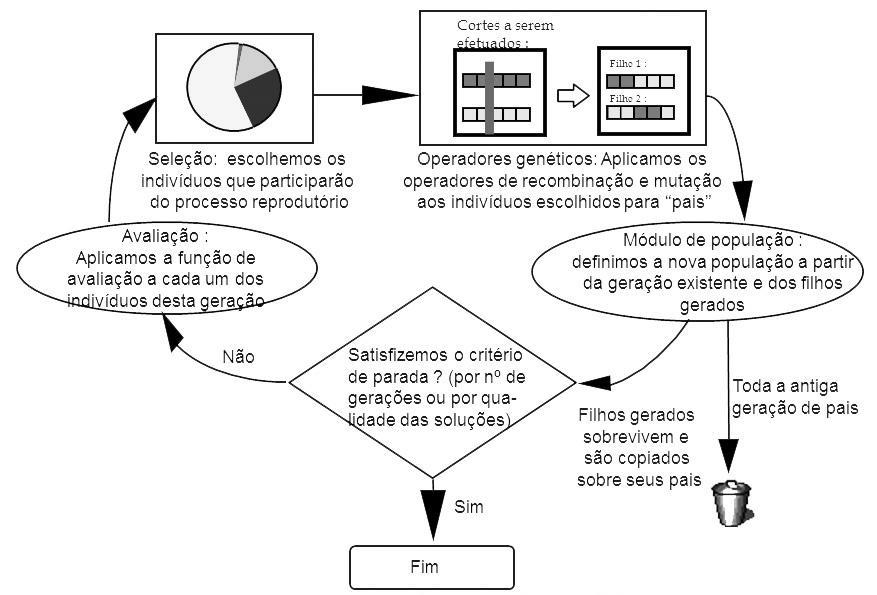
\includegraphics[scale=0.6]{imagens/nome-cap/nome-sec/esquemaAlgGenetico_pag64.png}
	\legend{Fonte: \citeonline[p. 64]{linden2012}.}
    	\end{center}
    \end{figure}
    
Incluindo uma figura de autoria própria.
\begin{figure} [htb]
\begin{center}
	 \caption{\label{fig:ambiente}Ambiente abordado}
	    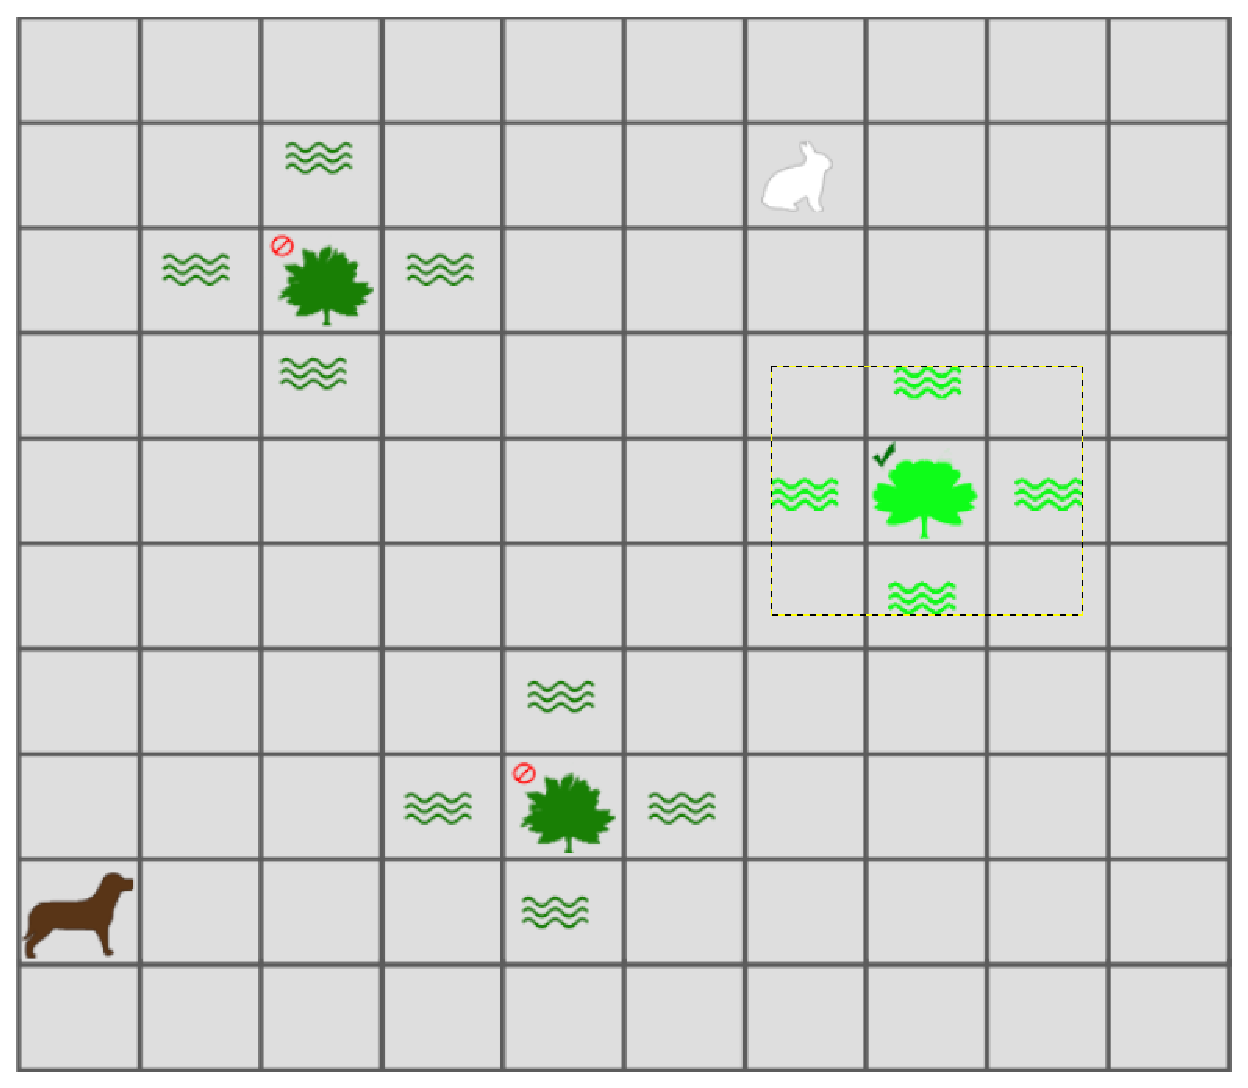
\includegraphics[scale=0.3]{imagens/nome-cap/nome-sec/ambiente.eps}
	\legend{Fonte: autoria própria.}
    \end{center}
\end{figure}


% %%%%%%%%%%%%%%%%%%%%%%%%%%%%%%%%%%%%%%%%%%%%%%%%%%%%%%%%%%%%%%%%%%%%%%%%%
\chapter{Desenvolvimento} \label{ch:definir-um-label-titulo-de-capitulo}
% %%%%%%%%%%%%%%%%%%%%%%%%%%%%%%%%%%%%%%%%%%%%%%%%%%%%%%%%%%%%%%%%%%%%%%%%%
A parte referente ao ``Desenvolvimento'' pode ser dividido em dois ou mais capítulos, e cada capítulo pode ser dividido em seções e subseções caso seja necessário para melhorar a apresentação e a legibilidade do documento.

Para referenciar a tabela você pode usar o comando "autoref" ex: \autoref{tab:resultados1}, ou o "ref", ex: \ref{tab:resultados1}

\begin{table}[htb]
\centering
\caption{Exemplo de tabela conforme a ABNT}
\label{tab:resultados1}
\begin{tabular}{p{0.3\textwidth} p{0.3\textwidth} p{0.3\textwidth}} % Ajuste das larguras das colunas
    \hline
    \textbf{Coluna 1} & \textbf{Coluna 2} & \textbf{Coluna 3} \\
    \hline
    Informação 1 & Informação 2 & Informação 3 \\
    Informação 4 & Informação 5 & Informação 6 \\
    Informação 7 & Informação 8 & Informação 9 \\  
    \hline
\end{tabular}
\legend{Fonte: autoria própria.}
\end{table}

\begin{table}[htb]
\centering
\caption{Exemplo de tabela conforme a ABNT}
\label{tab:resultados2}
\begin{tabular}{>{\centering\arraybackslash}p{0.3\textwidth}  >{\centering\arraybackslash}p{0.3\textwidth}  >{\centering\arraybackslash}p{0.3\textwidth}} % Ajuste das larguras das colunas
    \hline
    \textbf{Coluna 1} & \textbf{Coluna 2} & \textbf{Coluna 3} \\
    \hline
    Informação 1 & Informação 2 & Informação 3 \\
    Informação 4 & Informação 5 & Informação 6 \\
    Informação 7 & Informação 8 & Informação 9 \\  
    \hline
\end{tabular}
\legend{Fonte: autoria própria.}
\end{table}




\begin{table}[h]
    \centering
    \caption{Exemplo de tabela conforme a ABNT}
    \label{quad:exemplo}
    \begin{tabular}{p{3cm} p{4cm} p{3cm}}
        \hline%\toprule
        \textbf{Coluna 1} & \textbf{Coluna 2} & \textbf{Coluna 3} \\
        \hline%\midrule
        Informação 1 & Informação 2 & Informação 3 \\
        Informação 4 & Informação 5 & Informação 6 \\
        Informação 7 & Informação 8 & Informação 9 \\
        \hline%\bottomrule
    \end{tabular}
    \legend{Fonte: \citeonline{linden2012}.}
\end{table}

% %%%%%%%%%%%%%%%%%%%%%%%%%%%%%%%%%%%%%%%%%%%%%%%%%%%%%%%%%%%%%%%%%%%%%%%%%
\chapter{Conclusão} \label{ch:conclusao}
% %%%%%%%%%%%%%%%%%%%%%%%%%%%%%%%%%%%%%%%%%%%%%%%%%%%%%%%%%%%%%%%%%%%%%%%%%

A conclusão deve apresentar um resumo das principais descobertas do trabalho, avaliação do cumprimento do objetivos propostos na seção \textbf{objetivos} e possíveis sugestões para trabalhos futuros.

% ******************************************************************************
%				           ELEMENTOS PÓS-TEXTUAIS				               *
% ******************************************************************************
\postextual
% ----------------------------------------------------------
\bibliography{referencias}

% **********************************************************
%				  ELEMENTOS PÓS-TEXTUAIS				   *
% **********************************************************


% ----------------------------------------------------------
% Glossário
% ----------------------------------------------------------
%
% Consulte o manual da classe abntex2 para orientações sobre o glossário.
%
%\glossary

% ----------------------------------------------------------
% Apêndices
% ----------------------------------------------------------

% ---
% Inicia os apêndices
% ---
%\begin{apendicesenv}

% Imprime uma página indicando o início dos apêndices
%\partapendices

% ----------------------------------------------------------
%\chapter{Quisque libero justo}
% ----------------------------------------------------------

%\lipsum[50]

% ----------------------------------------------------------
%\chapter{Nullam elementum urna vel imperdiet sodales elit ipsum pharetra ligula
%ac pretium ante justo a nulla curabitur tristique arcu eu metus}
% ----------------------------------------------------------
%\lipsum[55-57]

%\end{apendicesenv}
% ---


% ----------------------------------------------------------
% Anexos
% ----------------------------------------------------------

% ---
% Inicia os anexos
% ---
%\begin{anexosenv}

% Imprime uma página indicando o início dos anexos
%\partanexos

% ---
%\chapter{Morbi ultrices rutrum lorem.}
% ---
%\lipsum[30]

% ---
%\chapter{Cras non urna sed feugiat cum sociis natoque penatibus et magnis dis
%parturient montes nascetur ridiculus mus}
% ---

%\lipsum[31]

% ---
%\chapter{Fusce facilisis lacinia dui}
% ---

%\lipsum[32]

%\end{anexosenv}

%---------------------------------------------------------------------
% INDICE REMISSIVO
%---------------------------------------------------------------------
%\phantompart
%\printindex
%---------------------------------------------------------------------



% ------------ fim do documento ------------
\end{document}